\documentclass[tikz]{standalone}

\usepackage[english,russian]{babel}
\usepackage[T2A,T1]{fontenc}
\usepackage[utf8]{inputenc}

\usepackage
    {
        tikz,
        pgfplots,
        verbatim,
    }
\usetikzlibrary
    {
        arrows,
        patterns,
        angles,
        quotes,
        calc, 
        3d,  
        backgrounds, 
        positioning
    }
\tikzset
    {
        media/.style={font={\footnotesize\sffamily}},
        wave/.style={
            decorate,decoration={snake,post length=1.4mm,amplitude=2mm,
                segment length=1mm},thick},   
    }
\begin{document}
\begin{tikzpicture}
	% Round rectangle
	% \fill[gray!10,rounded corners] (0,-1) rectangle ++(10,1);
		
	\begin{scope}[xshift=0cm]
		\draw (0,0.5) rectangle node[above, yshift=1em] {1} ++(1,0.5);
		% \draw (0.5,0.5) -- (0.5,0);
		% \draw[blue,line width=.5pt,interface] (0,0) -- ++(1,0);    
	\end{scope}
		
	\draw[magenta, line width=2pt] (1,0.75) -- ++ (1,0);  
	% \draw [red,  line width=1pt] (1.5,0.75) circle (4pt);
	% \draw [->,red, line width=1pt] (1.5,0.5) -- ++ (0,0.6);
	\draw [->,red, line width=1pt] (3,0.5) -- ++ (0,0.6);
	\draw[magenta, line width=1pt] (2.5,0.75) -- ++ (2,0);  
	\draw[magenta, line width=1pt] (5.5,0.75) -- ++ (1.5,0);  
	\draw[magenta, line width=0.5pt] (7.5,0.75) -- ++ (1.5,0);  
	
	\begin{scope}[xshift=2cm]
		\xdef\len{0.5cm}
		\draw (0,0.5) rectangle node[above, yshift=1em] {2} ++(\len,0.5);
		\draw (0,0.5) -- ++(\len,0.5);
		% \draw (\len/2,0.5) -- (\len/2,0);
		% \draw[blue,line width=.5pt,interface] (0,0) -- ++(\len,0);    
	\end{scope}    
	
	\begin{scope}[xshift=4.5cm]
		\draw[draw=none] (-1,0.25) rectangle node[above, yshift=2em] {3} ++(3,1);
		\draw[line width=6pt] (-1,0.25) coordinate (1) -- ++(3,0)  coordinate (2);
		\draw[line width=6pt] (-1,1.25) coordinate (1') -- ++(3,0)  coordinate (2');

        \draw[densely dashed] ($(1)+(0.24pt,0)$) -- ($(1')+(0.24pt,0)$);
        \draw[densely dashed] ($(2)-(0.24pt,0)$) -- ($(2')-(0.24pt,0)$);
				
		% \pgftext{\includegraphics[width=150pt]{pic1.png}} at (0pt,0pt);
				
		\begin{scope}[xshift=-1.2cm, yshift=2.5cm]
			\begin{axis}[
					xlabel={$z$, мм},
					ylabel={$B$, Тл},
					scale=0.5,
					grid=both,
					grid style={line width=.1pt, draw=gray!10},
					major grid style={line width=.2pt,draw=gray!50},
					minor y tick num=4,
					minor x tick num=4,   
					xtick distance=20,
					ytick distance=.5,
					ymax = 1.8,
					xmin = -40,
					xmax = 40,
					ticklabel style={font=\tiny,fill=white},    
					axis lines=middle,     
					every axis x label/.style={
						at={(ticklabel* cs:1.05)},
						anchor=west,
					},
					every axis y label/.style={
						at={(ticklabel* cs:1.05)},
						anchor=south,
					},    
					/pgf/number format/.cd,
					use comma,
					set decimal separator={.},
					1000 sep={}, 
				]  
				\addplot[smooth] table [x=l, y=10t, col sep=tab] {../data/b_x.csv}; 
			\end{axis}    
		\end{scope}
				
				
		\draw (0,0.5) rectangle node[above, yshift=-.58em] {7} ++(1,0.5);
		% \draw (0.5,0.25) -- (0.5,0);
		% \draw[blue,line width=.5pt,interface] (0,0) -- ++(1,0);    
	\end{scope}  
		
	\begin{scope}[xshift=7cm]
		\xdef\len{0.5cm}
		\draw (0,0.5) rectangle node[above, yshift=1em] {4} ++(\len,0.5);
		\draw (0,0.5) -- ++(\len,0.5);
		% \draw (\len/2,0.5) -- (\len/2,0);
		% \draw[blue,line width=.5pt,interface] (0,0) -- ++(\len,0);    
	\end{scope} 
		
	\begin{scope}[xshift=9cm]
		\xdef\len{1cm}
		\draw (0,0.5) rectangle node[above, yshift=1em] {6} ++(\len,0.5);
		% \draw (\len/2,0.5) -- (\len/2,0);
		% \draw[blue,line width=.5pt,interface] (0,0) -- ++(\len,0);    
	\end{scope}      
		
		
	\begin{scope}[xshift=8.1cm]
		\xdef\len{0.25cm}
		\draw[fill=white] (0,0.5) rectangle node[above, yshift=1em] {5} ++(\len,0.5);
		% \draw (\len/2,0.5) -- (\len/2,0);
		% \draw[blue,line width=.5pt,interface] (0,0) -- ++(\len,0);    
	\end{scope}           
	% \draw[-latex,thick](5.25,0.5)node[right]{}
	% ..controls +(180:.2cm) and +(up:0.25cm) .. (5,0);

	\node[anchor=south west, inner sep=0pt, outer sep=0pt, scale=0.261]
  (image) at (-1.7,2.05) {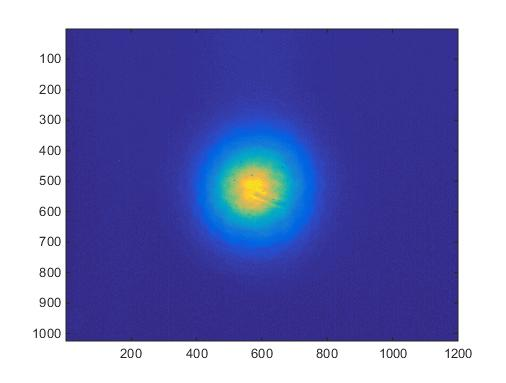
\includegraphics{1}};

	\node[anchor=south west, inner sep=0pt, outer sep=0pt, scale=0.261]
  (image) at (7,2.05) {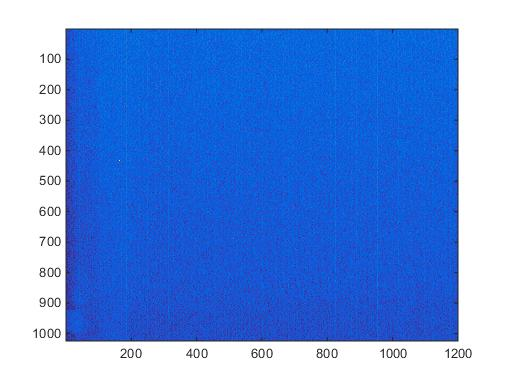
\includegraphics{2}};
  % xshift=-1.2cm, yshift=2.5cm
\end{tikzpicture} 
\end{document}